\documentclass[border=3pt,tikz]{standalone}
% Shared look for every TikZ figure in these notes.
% Included by each standalone figure file; also keeps the figures consistent
% with the colours used in the PDF and on the website.

\usepackage{tikz}
\usepackage{pgfplots}
\pgfplotsset{compat=1.18}
\usetikzlibrary{arrows.meta, decorations.markings, decorations.pathmorphing,
                patterns, calc, positioning}
\usepackage{amsmath}

% Series colours are the three validated categorical slots also used by the
% interactive widgets, so a path drawn in the printed notes and the same path on
% the website are the same colour. They clear the colour-vision-deficiency and
% contrast checks as a set; every path is direct-labelled as well, so colour is
% never the only thing carrying identity.
\definecolor{duPurple}{HTML}{68246D}
\definecolor{duBlue}{HTML}{2A78D6}
\definecolor{duRed}{HTML}{EB6834}
\definecolor{duGreen}{HTML}{1BAF7A}
\definecolor{duGrey}{HTML}{6B6B6B}

\tikzset{
  axisline/.style   = {-{Stealth[length=3mm]}, line width=0.7pt, black},
  path1/.style      = {duBlue,   line width=1.1pt},
  path2/.style      = {duRed,    line width=1.1pt},
  path3/.style      = {duGreen,  line width=1.1pt},
  statedot/.style   = {circle, fill=black, inner sep=1.4pt},
  arrowhead/.style  = {decoration={markings,
                        mark=at position #1 with {\arrow{Stealth[length=2.6mm]}}},
                       postaction={decorate}},
  lbl/.style        = {font=\small},
  slbl/.style       = {font=\footnotesize, duGrey},
  workfill/.style   = {duPurple, opacity=0.16},
}

% reversible process: area under P-V path is |W|, area under T-S path is |Q|
\begin{document}
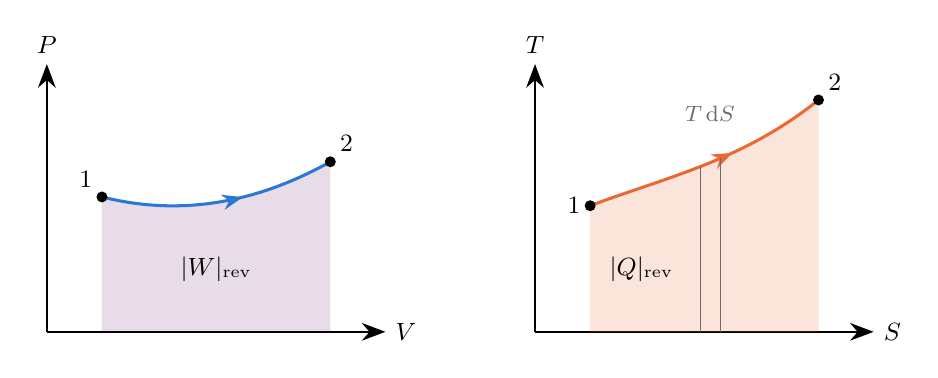
\begin{tikzpicture}[x=1cm,y=1cm]
  % P-V
  \draw[axisline] (0,0) -- (4.3,0) node[right, lbl] {$V$};
  \draw[axisline] (0,0) -- (0,3.4) node[above, lbl] {$P$};
  \fill[workfill] (0.7,0) -- plot[domain=0.7:3.6, samples=40] (\x,{1.6+0.14*(\x-1.6)^2}) -- (3.6,0) -- cycle;
  \draw[path1, arrowhead=0.6] plot[domain=0.7:3.6, samples=40] (\x,{1.6+0.14*(\x-1.6)^2});
  \node[statedot] at (0.7,1.713) {}; \node[lbl, above left] at (0.7,1.713) {1};
  \node[statedot] at (3.6,2.16) {};  \node[lbl, above right] at (3.6,2.16) {2};
  \node[lbl] at (2.15,0.8) {$|W|_\text{rev}$};
  % T-S
  \begin{scope}[shift={(6.2,0)}]
  \draw[axisline] (0,0) -- (4.3,0) node[right, lbl] {$S$};
  \draw[axisline] (0,0) -- (0,3.4) node[above, lbl] {$T$};
  \fill[duRed, opacity=0.18] (0.7,0) -- plot[domain=0.7:3.6, samples=40] (\x,{1.3+0.5*\x-0.12*\x^2+0.03*\x^3}) -- (3.6,0) -- cycle;
  \draw[path2, arrowhead=0.6] plot[domain=0.7:3.6, samples=40] (\x,{1.3+0.5*\x-0.12*\x^2+0.03*\x^3});
  \draw[duGrey] (2.1,0) -- (2.1,{1.3+0.5*2.1-0.12*2.1^2+0.03*2.1^3});
  \draw[duGrey] (2.35,0) -- (2.35,{1.3+0.5*2.35-0.12*2.35^2+0.03*2.35^3});
  \node[slbl, above] at (2.22,2.55) {$T\,\mathrm{d}S$};
  \node[statedot] at (0.7,{1.3+0.35-0.0588+0.0103}) {}; \node[lbl, left] at (0.7,1.6) {1};
  \node[statedot] at (3.6,{1.3+1.8-1.5552+1.39968}) {}; \node[lbl, above right] at (3.6,2.94) {2};
  \node[lbl] at (1.35,0.8) {$|Q|_\text{rev}$};
  \end{scope}
\end{tikzpicture}
\end{document}
